In this section we empirically demonstrate that our CASH mechanism can be used to significantly reduce the fraction of accounts that an offline adversary could compromise. We implemented Algorithm \ref{alg:HeuristicAlg2} in C\# using Gurobi as our LP solver, and analyzed CASH using two real-world password distributions $p_1,\ldots,p_n$. The first distribution is based on data from the RockYou password breach ($32+$ million passwords) and the second is based on password frequency data from Yahoo! users (representing $\approx 70$ million passwords). The later dataset was not the result of a security breach. Instead, Yahoo! gave Bonneau~\cite{bonneau2012science} permission to collect and analyze password frequency data in a carefully controlled environment. Yahoo! recently allowed Blocki et al.~\cite{blocki2016differentially} to use a differentially private~\cite{dwork2006calibrating} algorithm to publish this data. Thus, the password frequency data in this data set has been perturbed slightly.  Blocki et al.~\cite{blocki2016differentially} also showed that with high probability the L1 error introduced by their algorithm would be minimal. 


In each of our experiments we fix the password correctness rate $\alpha \in \{1,0.95,0.9\}$ and the maximum amortized server cost $C_{max}$ before using Algorithm \ref{alg:HeuristicAlg2} to find a CASH parameters $\tilde{p}_1,\ldots, \tilde{p}_m$ and $k$ subject to the appropriate constraints on the amortized server costs. 

We compare the $\%$ of cracked passwords under three different scenarios: 
\begin{itemize}
\item (Deterministic Key-Stretching) The authentication server selects a hash function $\Hash^k$  with cost parameter  $k = C_{max}$ (achieved through traditional deterministic key-stretching techniques). The rational value $v$ adversary will crack each password with probability $\PAdvDet{v}{k}$ (eq \ref{eq:PAdvDet}).   
\item (Uniform-CASH) The authentication server uses CASH with the uniform distribution. He sets $k$ according to eq \ref{eq:kUnifCash}
to ensure that his amortized costs are at most $C_{max}$. A rational value $v$ adversary will crack each password with probability $\PAdvUnif{v}{C_{max}}$. 

\item (CASH) Given an estimate $\hat{v}$ of the adversary's budget we used Algorithm \ref{alg:HeuristicAlg2} to optimize the CASH parameters $k$ and $\tilde{p}_1,\ldots, \tilde{p}_m$ subject to the constraint that the amortized server cost is at most $C_{max}$ when users enter the wrong password with probability $1-\alpha$. We fixed the parameters $m=50, \epsilon = 0.02$, and we set $\mathcal{B} = \{5\cdot C_{max} \times 10^4$, $C_{max}\times 10^6$, $C_{max}\times 10^7$, $1.5\cdot C_{max}\times 10^7$, $2.0\cdot C_{max} \times 10^7$,  $2.5\cdot C_{max} \times 10^7$, $2.65\cdot C_{max} \times 10^7$, $2.8\cdot C_{max} \times 10^7$, $3.0\cdot C_{max} \times 10^7$, $5.0\cdot C_{max} \times 10^7$, $C_{max} \times 10^8\}$. Thus, Algorithm \ref{alg:HeuristicAlg2} computes the optimal distribution against a threshold $B$ adversary for each $B \in \mathcal{B}$, and selects the best distribution $\tilde{p}$ against a value $\hat{v}$ adversary.  $\PAdvCASH{\hat{v}}{\hat{v}}{C_{max}}$ will denote the fraction of cracked passwords when the true value is $v=\hat{v}$. When the adversary's true value is $v \neq \hat{v}$, $\PAdvCASH{v}{\hat{v}}{C_{max}}$  will denote the fraction of cracked passwords.  
\end{itemize}

Our results indicate that an authentication server could significantly reduce the fraction of compromised passwords in an offline attack by adopting our optimal CASH mechanism instead of deterministic key-stretching or uniform-CASH. These results held robustly for both the RockYou and Yahoo! password distributions.






\subsubsection{Password Datasets} \label{subsubsec:RockYou} We use two password frequency datasets, RockYou and Yahoo!, to analyze our CASH mechanism. The RockYou dataset contains passwords from $N\approx 32.6$ million RockYou users, and the Yahoo! dataset contains data from $N\approx 70$ million Yahoo! users. We used frequency data from each of these datasets to obtain an empirical password distribution $p_1 \geq p_2 \geq p_3 \ldots \geq p_n$ over $\PasswordSpace$. 

The RockYou dataset is based on actual user passwords which were leaked during the infamous RockYou security breach (RockYou had been storing these passwords in the clear). The total number of unique passwords in the dataset was $n \approx 14.3$ million. Approximately, $11.9$ million of these passwords were unique to one RockYou user. The other $\approx 2.5$ million passwords were used by multiple users. The most popular password ($pwd_1=$ `123456') was shared by $\approx 0.3$ million RockYou users ($p_1 \approx 0.01$). RockYou did not impose strict password restrictions on its users (e.g. users were allowed to select passwords consisting of only lowercase letters or only numbers). 

We also used (perturbed) password frequency data from a dataset of $N\approx 70$ million Yahoo! passwords. See~\cite{bonneau2012science} for more details about how this data was collected and see~\cite{blocki2016differentially} for more details about how the frequency data was perturbed to satisfy the rigorous notion of differentially privacy~\cite{dwork2006calibrating}. Blocki et al.~\cite{blocki2016differentially} proved that with high probability the L1 distortion of the perturbed frequency data is bounded by $O\left( \sqrt{N}/\epsilon\right)$, where the privacy parameter was set to $\epsilon=0.25$ when the Yahoo! dataset was published. Thus, the perturbed dataset will also still give us a good estimate of the empirical password distribution.  

\cut{
\subsubsection{Comparing Defenses}
Given fixed values $B, \alpha,$ and $C_{SRV,\alpha}$ it is critically important to make a fair comparison between the different defenses that the authentication server might adopt. If the authentication server adopts a deterministic key-stretching algorithm $\mathbf{H}^{k'}$ then he can afford to set $k'= C_{SRV,\alpha}$ so that his average cost per authentication is $C_{SRV,\alpha}$. In this case the adversary can guess $B/k'$ passwords (to simplify presentation we assume that $k'$ divides $B$) so we have \[\mathcal{P}_{ADV,B} = \sum_{i=1}^{\lfloor B/k' \rfloor} p_i \ . \]
Similarly, if the authentication server adopts the uniform-CASH strategy with $k=1$ then he can afford to set 
\[m' = \frac{2\cdot C_{SRV,\alpha} - \alpha}{2-\alpha} \approx  \frac{2\cdot C_{SRV,\alpha}}{2-\alpha} \ , \]
so that his average cost per login is at most $C_{SRV,\alpha}$. 
In this case we will have \[\mathcal{P}_{ADV,B} = \sum_{i=1}^{ B/m' } p_i  \ , \]
because the adversary's optimal strategy is to spend all of his budget guessing the $B/m'$ most popular passwords. Finally, if the authentication server adopts our CASH mechanism then he will run algorithm \ref{alg:HeuristicAlg} with the fixed values $B, \alpha, C_{SRV,\alpha}$ to obtain $m^*,k^*,\tilde{p}_1,\ldots,\tilde{p}_m$. The algorithm is guaranteed to find a solution in which the average cost at most $C_{SRV,\alpha}$. In this case the adversary's success rate is 
\[\mathcal{P}_{ADV,B} = \max_{b \in \mathcal{F}_B} \sum_{i=1}^{n} \sum_{j=1}^{b_i} p_i\cdot\tilde{p}_j \ .\]


\subsubsection{Parameter Selection} \label{subsubsec:ParameterTuning}
In each experiment we fixed the ratio $\frac{B}{C_{SRV,\alpha}}$, the ratio between the work that the offline adversary is willing to do and the work that a legitimate authentication server needs to do on average. If the authentication server uses $k' = C_{SRV,\alpha}$ rounds of deterministic key-stretching then $\frac{B}{C_{SRV,\alpha}}$ denotes the total number of password guesses that the offline adversary can try. In our experiments, we considered the following range of values for this ratio $\frac{B}{C_{SRV,\alpha}}$: $\{10^2, 5\times 10^2, 10^3, 5\times 10^3, 10^4, 5 \times 10^4, 10^5, 5\times 10^5, 10^6, 5 \times 10^6, 10^7, 10^7 + 5\times 10^6, \ldots, 2 \times 10^7, 2.5\times 10^7, 2.65 \times 10^7, 2.8 \times 10^7\}$.  We expect that the adversary's success rate  $\mathcal{P}_{ADV,B}$ will increase as this ratio increases --- a server that is willing to do more work on average during authentication can better protect its users. 

When selecting $k$ and $m$ we need to ensure that $(1-\alpha)km < C_{SRV,\alpha}$. In general, we get more flexibility in our optimization problem by selecting $m$ large and then selecting $k < \frac{C_{SRV,\alpha}}{m(1-\alpha)}$. However, the optimization problem becomes harder to solve as $m$ increases. Thus, we fixed $m=50$ when optimizing CASH while allowing $k$ to vary because we could not find any noticeable improvement in obtained CASH solutions for $m > 50$. We used our CASH optimization algorithm to optimize the value and $k$ as well as $\tilde{p}_1,\ldots,\tilde{p}_m$. }


\subsection{Results}
Our first set of experimental results are shown in Figures \ref{fig:YahooResults1} and \ref{fig:RockYouResults1}. These plots were computed under the assumption that $\alpha = 1$ (users always enter their passwords correctly), and that $\hat{v}=v$ (the defender knows the exact adversary value). The results show that for some (higher) adversary values our non-uniform CASH distributions improves significantly on the cost-equivalent versions of uniform CASH ($50\%$ reduction in cracked passwords) and deterministic key-stretching ($56\%$ reduction in cracked passwords).\footnote{We note that we would expect to see relatively high adversary  values $v/C_{max}$ in the offline setting because $C_{max}$ will typically be quite small (e.g., $\$10^{-6}$). }  Figures \ref{fig:YahooResults90} and \ref{fig:RockYouResults90} (resp. Figures \ref{fig:YahooResults95} and \ref{fig:RockYouResults95}) show the same results under the assumptions that $\alpha = 0.9$ (resp. $\alpha=0.95$). 

Figures \ref{fig:YahooRobust2Results95} and \ref{fig:YahooRobust1Results95} (resp. Figures \ref{fig:RockYouRobust1Results95} and \ref{fig:RockYouRobust2Results95}) explore the effect of a wrong estimate $\hat{v} \neq v$ of the adversary's value for both the RockYou and Yahoo! datasets. Despite receiving the wrong estimate $\hat{v}$ our algorithm returns a distribution that is (almost always) slightly better than the corresponding uniform CASH distribution. Both distributions still significantly outperform the cost equivalent deterministic key-stretching solution. 

\FullVersion{The full version~\cite{fullVersion} of this paper contains additional plots exploring what happens when the defender uses the wrong empirical password distribution when searching for a good CASH distribution $\tilde{p}$ (e.g., if the defender optimizes $\tilde{p}$ under the assumption that the empirical password distribution is given by the Yahoo! dataset when the actual distribution is given by the RockYou dataset).
}{Figures \ref{fig:RockYouResultsOptForYahoo95} and  \ref{fig:YahooResultsOptForRockYou95}  in the appendix explore what happens when the defender uses the wrong empirical password distribution when searching for a good CASH distribution $\tilde{p}$ (e.g., if the defender optimizes $\tilde{p}$ under the assumption that the empirical password distribution is given by the Yahoo! dataset when the actual distribution is given by the RockYou dataset). } Briefly, these plots show that non-uniform CASH significantly outperforms deterministic key-stretching even when non-uniform CASH is optimized under the wrong distribution and non-uniform CASH slightly outperforms uniform CASH on most, but not all, of the curve. 


\begin{figure}[!t]
\centering
    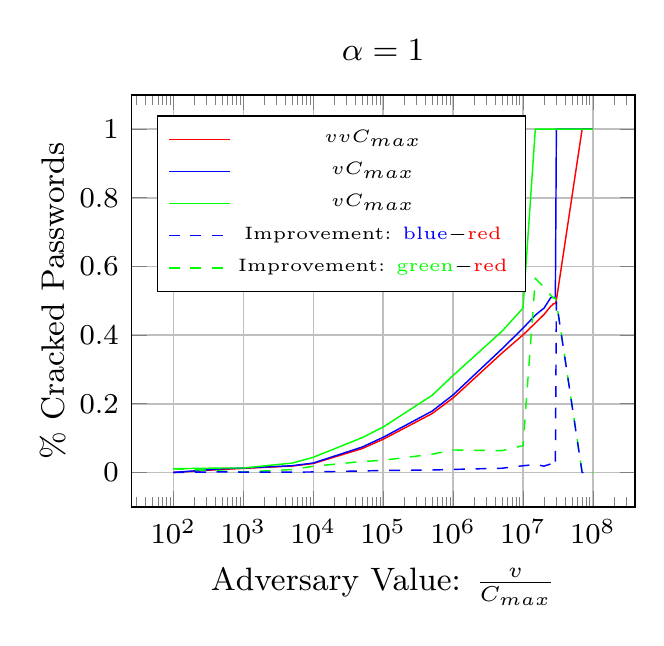
\begin{tikzpicture}[scale=1.3]  
   \begin{semilogxaxis}[
    title style={align=center},
    title={ {\small $\alpha=1$ }},
    xlabel={Adversary Value: $\frac{v}{C_{max}}$},
    ylabel={$\%$ Cracked Passwords},
    ylabel shift = -3pt,
grid=major,
    small,
    cycle list = {{red, mark=none}, {blue, mark=none}, {green, mark=none},{green, dashed, mark=none}, {blue, dashed, mark=none},  {blue, dashed, mark=none}, {red, dashed, mark=none},{brown, dashed, mark=none} },
    legend style = {font=\tiny, at={(.05,.95)}, anchor=north west},
    legend entries = { $\PAdvCASH{v}{v}{C_{max}}$, $\PAdvUnif{v}{C_{max}}$, $\PAdvDet{v}{C_{max}}$, Improvement: \textcolor{blue}{blue}$-$\textcolor{red}{red}, Improvement: \textcolor{green}{green}$-$\textcolor{red}{red}}
   ] 

    \addlegendimage{no markers, red, mark=square*}
    \addlegendimage{no markers, blue, mark=square*}
    \addlegendimage{no markers, green, mark=square*}
    \addlegendimage{no markers, dashed, blue}
    \addlegendimage{no markers, dashed, green}
\addplot coordinates {  (100,0)  (500,0.00901095679831186)  (1000,0.0118882075379984)  (5000,0.0187377670340035)  (10000,0.0260329771951511)  (50000,0.0695289722433699)  (100000,0.0967762178707898)  (500000,0.171395066946001)  (1000000,0.217079290083012)  (5000000,0.347777554099186)  (10000000,0.400698912520617)  (15000000,0.435241555034486)  (20000000,0.460298959755672)  (25000000,0.484752773595168)  (26500000,0.487934163505628)  (27000000,0.491586385753338)  (27500000,0.491586385753338)  (28000000,0.491891527286909)  (29000000,0.491904229037079)  (30000000,0.501829516819533)  (70000000,0.999999999999975)  (100000000,0.999999999999975)  };
\addplot coordinates {  (100,0)  (500,0.0108687224894377)  (1000,0.0130192581998815)  (5000,0.0196877875530742)  (10000,0.0275769138479969)  (50000,0.0740168548263362)  (100000,0.102497142299001)  (500000,0.178594664053884)  (1000000,0.225985726653441)  (5000000,0.360129776428412)  (10000000,0.420317345392629)  (15000000,0.45834913690049)  (20000000,0.478853387778074)  (25000000,0.50975028086399)  (26500000,0.50975028086399)  (27000000,0.50975028086399)  (27500000,0.50975028086399)  (28000000,0.50975028086399)  (29000000,0.50975028086399)  (30000000,1)  (70000000,1)  (100000000,1)  };
\addplot coordinates {  (100,0.0108687224894377)  (500,0.0130192581998815)  (1000,0.0130192581998815)  (5000,0.0273838584095427)  (10000,0.0441510096695537)  (50000,0.101412040578669)  (100000,0.132372669808665)  (500000,0.224601121331902)  (1000000,0.282624504055384)  (5000000,0.411368138539665)  (10000000,0.478853387778074)  (15000000,1)  (20000000,1)  (25000000,1)  (26500000,1)  (27000000,1)  (27500000,1)  (28000000,1)  (29000000,1)  (30000000,1)  (70000000,1)  (100000000,1)  };
\addplot coordinates {  (100,0.0108687224894377)  (500,0.00400830140156962)  (1000,0.0011310506618831)  (5000,0.00864609137553916)  (10000,0.0181180324744026)  (50000,0.0318830683352988)  (100000,0.0355964519378749)  (500000,0.0532060543859009)  (1000000,0.0655452139723718)  (5000000,0.0635905844404786)  (10000000,0.0781544752574576)  (15000000,0.564758444965514)  (20000000,0.539701040244328)  (25000000,0.515247226404832)  (26500000,0.512065836494372)  (27000000,0.508413614246662)  (27500000,0.508413614246662)  (28000000,0.508108472713091)  (29000000,0.508095770962921)  (30000000,0.498170483180467)  (70000000,2.48689957516035E-14)  (100000000,2.48689957516035E-14)  };
\addplot coordinates {  (100,0)  (500,0.00185776569112582)  (1000,0.0011310506618831)  (5000,0.000950020519070692)  (10000,0.00154393665284583)  (50000,0.00448788258296633)  (100000,0.00572092442821077)  (500000,0.0071995971078832)  (1000000,0.00890643657042919)  (5000000,0.0123522223292253)  (10000000,0.0196184328720127)  (15000000,0.0231075818660044)  (20000000,0.0185544280224019)  (25000000,0.0249975072688218)  (26500000,0.0218161173583619)  (27000000,0.0181638951106518)  (27500000,0.0181638951106518)  (28000000,0.0178587535770803)  (29000000,0.0178460518269108)  (30000000,0.498170483180467)  (70000000,2.48689957516035E-14)  (100000000,2.48689957516035E-14)  };


   \end{semilogxaxis} 
  \end{tikzpicture}
  
  \caption{Yahoo Dataset: $\alpha = 1$.}
\label{fig:YahooResults1}
\end{figure}
 
\begin{figure}[!t]
\centering
    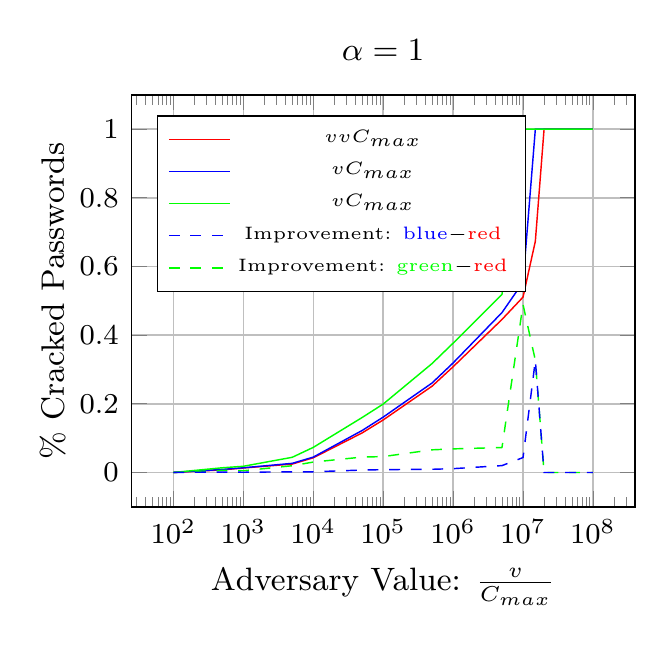
\begin{tikzpicture}[scale=1.3]  
   \begin{semilogxaxis}[
    title style={align=center},
    title={ {\small $\alpha=1$ }},
    xlabel={Adversary Value: $\frac{v}{C_{max}}$},
    xlabel={Adversary Value: $\frac{v}{C_{max}}$},
    ylabel={$\%$ Cracked Passwords},
    ylabel shift = -3pt,
grid=major,
    small,
    cycle list = {{red, mark=none}, {blue, mark=none}, {green, mark=none},{green, dashed, mark=none}, {blue, dashed, mark=none},  {blue, dashed, mark=none}, {red, dashed, mark=none},{brown, dashed, mark=none} },
    legend style = {font=\tiny, at={(.05,.95)}, anchor=north west},
    legend entries = { $\PAdvCASH{v}{v}{C_{max}}$, $\PAdvUnif{v}{C_{max}}$, $\PAdvDet{v}{C_{max}}$, Improvement: \textcolor{blue}{blue}$-$\textcolor{red}{red}, Improvement: \textcolor{green}{green}$-$\textcolor{red}{red}}
   ] 

    \addlegendimage{no markers, red, mark=square*}
    \addlegendimage{no markers, blue, mark=square*}
    \addlegendimage{no markers, green, mark=square*}
    \addlegendimage{no markers, dashed, blue}
    \addlegendimage{no markers, dashed, green}
\addplot coordinates {  (100,0)  (500,0.0076046384413692)  (1000,0.0130127814866306)  (5000,0.0245423032689714)  (10000,0.0427309815113077)  (50000,0.11520218186584)  (100000,0.15297695370972)  (500000,0.251342450785729)  (1000000,0.307887790562047)  (5000000,0.445734691700375)  (10000000,0.510814832636074)  (15000000,0.673482337523552)  (20000000,0.999999999999993)  (25000000,0.999999999999993)  (26500000,0.999999999999993)  (27000000,0.999999999999993)  (27500000,0.999999999999993)  (28000000,0.999999999999993)  (29000000,0.999999999999993)  (30000000,0.999999999999993)  (70000000,0.999999999999993)  (100000000,0.999999999999993)  };
\addplot coordinates {  (100,0)  (500,0.00891714075850031)  (1000,0.0136977788934083)  (5000,0.0265629142590948)  (10000,0.0447626485934529)  (50000,0.12227710813367)  (100000,0.161237660331497)  (500000,0.260629600825534)  (1000000,0.319035371416001)  (5000000,0.465731506185799)  (10000000,0.55428368364662)  (15000000,1)  (20000000,1)  (25000000,1)  (26500000,1)  (27000000,1)  (27500000,1)  (28000000,1)  (29000000,1)  (30000000,1)  (70000000,1)  (100000000,1)  };
\addplot coordinates {  (100,0)  (500,0.0136977788934083)  (1000,0.0180747779954648)  (5000,0.0441965417827129)  (10000,0.0730608733055595)  (50000,0.160089926850547)  (100000,0.199287847017616)  (500000,0.317302545367371)  (1000000,0.376634078642379)  (5000000,0.518411276766697)  (10000000,1)  (15000000,1)  (20000000,1)  (25000000,1)  (26500000,1)  (27000000,1)  (27500000,1)  (28000000,1)  (29000000,1)  (30000000,1)  (70000000,1)  (100000000,1)  };
\addplot coordinates {  (100,0)  (500,0.00609314045203905)  (1000,0.00506199650883418)  (5000,0.0196542385137415)  (10000,0.0303298917942517)  (50000,0.0448877449847074)  (100000,0.0463108933078961)  (500000,0.065960094581642)  (1000000,0.0687462880803322)  (5000000,0.0726765850663217)  (10000000,0.489185167363926)  (15000000,0.326517662476448)  (20000000,7.105427357601E-15)  (25000000,7.105427357601E-15)  (26500000,7.105427357601E-15)  (27000000,7.105427357601E-15)  (27500000,7.105427357601E-15)  (28000000,7.105427357601E-15)  (29000000,7.105427357601E-15)  (30000000,7.105427357601E-15)  (70000000,7.105427357601E-15)  (100000000,7.105427357601E-15)  };
\addplot coordinates {  (100,0)  (500,0.00131250231713111)  (1000,0.000684997406777665)  (5000,0.00202061099012341)  (10000,0.00203166708214515)  (50000,0.0070749262678306)  (100000,0.00826070662177641)  (500000,0.00928715003980463)  (1000000,0.0111475808539544)  (5000000,0.0199968144854238)  (10000000,0.0434688510105455)  (15000000,0.326517662476448)  (20000000,7.105427357601E-15)  (25000000,7.105427357601E-15)  (26500000,7.105427357601E-15)  (27000000,7.105427357601E-15)  (27500000,7.105427357601E-15)  (28000000,7.105427357601E-15)  (29000000,7.105427357601E-15)  (30000000,7.105427357601E-15)  (70000000,7.105427357601E-15)  (100000000,7.105427357601E-15)  };


   \end{semilogxaxis} 
  \end{tikzpicture}
  
  \caption{RockYou Dataset: $\alpha = 1$.}
\label{fig:RockYouResults1}
\end{figure} 
  
   \begin{figure}[!t]
   \centering
\subfloat[Yahoo]{
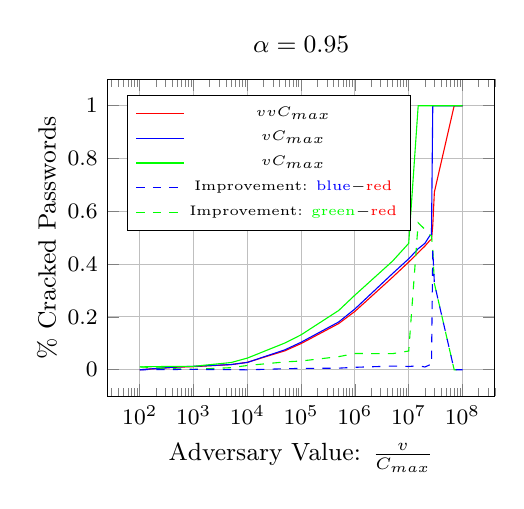
\begin{tikzpicture}[scale=1.0]  
   \begin{semilogxaxis}[
    title style={align=center},
    title={ {\small $\alpha=0.95$ }},
    xlabel={Adversary Value: $\frac{v}{C_{max}}$},
    ylabel={$\%$ Cracked Passwords},
    ylabel shift = -3pt,
grid=major,
    small,
    cycle list = {{red, mark=none}, {blue, mark=none}, {green, mark=none},{green, dashed, mark=none}, {blue, dashed, mark=none},  {blue, dashed, mark=none}, {red, dashed, mark=none},{brown, dashed, mark=none} },
    legend style = {font=\tiny, at={(.05,.95)}, anchor=north west},
    legend entries = { $\PAdvCASH{v}{v}{C_{max}}$, $\PAdvUnif{v}{C_{max}}$, $\PAdvDet{v}{C_{max}}$, Improvement: \textcolor{blue}{blue}$-$\textcolor{red}{red}, Improvement: \textcolor{green}{green}$-$\textcolor{red}{red}}
   ] 

    \addlegendimage{no markers, red, mark=square*}
    \addlegendimage{no markers, blue, mark=square*}
    \addlegendimage{no markers, green, mark=square*}
    \addlegendimage{no markers, dashed, blue}
    \addlegendimage{no markers, dashed, green}
\addplot coordinates {  (100,0)  (500,0.00974816549150774)  (1000,0.0115631568630905)  (5000,0.0194896102497567)  (10000,0.0280671385165211)  (50000,0.071791685890364)  (100000,0.0992383142594701)  (500000,0.175014737387696)  (1000000,0.221098434924485)  (5000000,0.35036457681152)  (10000000,0.407944399818817)  (15000000,0.443322031170548)  (20000000,0.468392975247313)  (25000000,0.490721988368897)  (26500000,0.492844202602487)  (28000000,0.546494585567765)  (30000000,0.673166853909312)  (70000000,0.999999999999971)  (100000000,0.999999999999971)  };
\addplot coordinates {  (100,0)  (500,0.0108687224894377)  (1000,0.0130192581998815)  (5000,0.0196877875530742)  (10000,0.0277625668318636)  (50000,0.0756145584896869)  (100000,0.104286400708258)  (500000,0.181055900840701)  (1000000,0.230322497241287)  (5000000,0.364249437207828)  (10000000,0.420317345392629)  (15000000,0.45834913690049)  (20000000,0.478853387778074)  (25000000,0.50975028086399)  (26500000,0.50975028086399)  (28000000,1)  (30000000,1)  (70000000,1)  (100000000,1)  };
\addplot coordinates {  (100,0.0108687224894377)  (500,0.0130192581998815)  (1000,0.0130192581998815)  (5000,0.0273838584095427)  (10000,0.0441510096695537)  (50000,0.101412040578669)  (100000,0.132372669808665)  (500000,0.224601121331902)  (1000000,0.282624504055384)  (5000000,0.411368138539665)  (10000000,0.478853387778074)  (15000000,1)  (20000000,1)  (25000000,1)  (26500000,1)  (28000000,1)  (30000000,1)  (70000000,1)  (100000000,1)  };
\addplot coordinates {  (100,0.0108687224894377)  (500,0.00327109270837374)  (1000,0.001456101336791)  (5000,0.00789424815978592)  (10000,0.0160838711530326)  (50000,0.0296203546883047)  (100000,0.0331343555491946)  (500000,0.0495863839442057)  (1000000,0.0615260691308984)  (5000000,0.0610035617281453)  (10000000,0.0709089879592568)  (15000000,0.556677968829452)  (20000000,0.531607024752687)  (25000000,0.509278011631104)  (26500000,0.507155797397513)  (28000000,0.453505414432235)  (30000000,0.326833146090688)  (70000000,2.89768209427166E-14)  (100000000,2.89768209427166E-14)  };
\addplot coordinates {  (100,0)  (500,0.00112055699792995)  (1000,0.001456101336791)  (5000,0.000198177303317452)  (10000,-0.000304571684657504)  (50000,0.00382287259932285)  (100000,0.00504808644878749)  (500000,0.00604116345300501)  (1000000,0.00922406231680187)  (5000000,0.0138848603963081)  (10000000,0.0123729455738119)  (15000000,0.0150271057299424)  (20000000,0.0104604125307615)  (25000000,0.0190282924950931)  (26500000,0.0169060782615023)  (28000000,0.453505414432235)  (30000000,0.326833146090688)  (70000000,2.89768209427166E-14)  (100000000,2.89768209427166E-14)  };

   \end{semilogxaxis} 
  \end{tikzpicture}

\label{fig:YahooResults95}}
\subfloat[Yahoo: $\hat{v}\neq v$]{   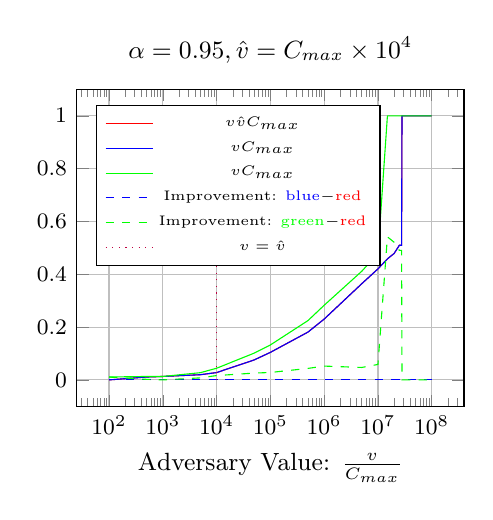
\begin{tikzpicture}[scale=1.0]  
   \begin{semilogxaxis}[
    title style={align=center},
    title={ {\small $\alpha=0.95, \hat{v} = C_{max}\times 10^4$ }},
       xlabel={Adversary Value: $\frac{v}{C_{max}}$},
ylabel shift = -3pt,
grid=major,
    small,
    cycle list = {{red, mark=none}, {blue, mark=none}, {green, mark=none},{blue, dashed, mark=none}, {green, dashed, mark=none},  {purple, dotted, mark=none}, {red, dashed, mark=none},{brown, dashed, mark=none} },
    legend style = {font=\tiny, at={(.05,.95)}, anchor=north west},
    legend entries = { $\PAdvCASH{v}{\hat{v}}{C_{max}}$, $\PAdvUnif{v}{C_{max}}$, $\PAdvDet{v}{C_{max}}$, Improvement: \textcolor{blue}{blue}$-$\textcolor{red}{red}, Improvement: \textcolor{green}{green}$-$\textcolor{red}{red}, $v = \hat{v}$  }
   ] 

    \addlegendimage{no markers, red, mark=square*}
    \addlegendimage{no markers, blue, mark=square*}
    \addlegendimage{no markers, green, mark=square*}
    \addlegendimage{no markers, dashed, blue}
    \addlegendimage{no markers, dashed, green}
    \addlegendimage{no markers, dotted, purple}
\addplot coordinates {  (100,0)  (500,0.0108687224894377)  (1000,0.0130192581998815)  (5000,0.0196877875530742)  (10000,0.0277625668318637)  (50000,0.0756145584896891)  (100000,0.104286400708252)  (500000,0.181055900840683)  (1000000,0.230322497241268)  (5000000,0.364249437207804)  (10000000,0.420317345392608)  (15000000,0.458349136900469)  (20000000,0.478853387778053)  (25000000,0.509750280863969)  (26500000,0.509750280863969)  (27000000,0.509750280863969)  (27500000,0.509750280863969)  (28000000,0.999999999999979)  (29000000,0.999999999999979)  (30000000,0.999999999999979)  (70000000,0.999999999999979)  (100000000,0.999999999999979)  };
\addplot coordinates {  (100,0)  (500,0.0108687224894377)  (1000,0.0130192581998815)  (5000,0.0196877875530742)  (10000,0.0277625668318636)  (50000,0.0756145584896869)  (100000,0.104286400708258)  (500000,0.181055900840701)  (1000000,0.230322497241287)  (5000000,0.364249437207828)  (10000000,0.420317345392629)  (15000000,0.45834913690049)  (20000000,0.478853387778074)  (25000000,0.50975028086399)  (26500000,0.50975028086399)  (27000000,0.50975028086399)  (27500000,0.50975028086399)  (28000000,1)  (29000000,1)  (30000000,1)  (70000000,1)  (100000000,1)  };
\addplot coordinates {  (100,0.0108687224894377)  (500,0.0130192581998815)  (1000,0.0130192581998815)  (5000,0.0273838584095427)  (10000,0.0441510096695537)  (50000,0.101412040578669)  (100000,0.132372669808665)  (500000,0.224601121331902)  (1000000,0.282624504055384)  (5000000,0.411368138539665)  (10000000,0.478853387778074)  (15000000,1)  (20000000,1)  (25000000,1)  (26500000,1)  (27000000,1)  (27500000,1)  (28000000,1)  (29000000,1)  (30000000,1)  (70000000,1)  (100000000,1)  };


\addplot coordinates {  (100,0)  (500,0)  (1000,1.38777878078145E-17)  (5000,-3.46944695195361E-18)  (10000,-1.38777878078145E-16)  (50000,-2.22044604925031E-15)  (100000,5.93969318174459E-15)  (500000,1.77358128183869E-14)  (1000000,1.8846035843012E-14)  (5000000,2.37587727269784E-14)  (10000000,2.17048601314218E-14)  (15000000,2.09832151654155E-14)  (20000000,2.07056594092592E-14)  (25000000,2.1094237467878E-14)  (26500000,2.1094237467878E-14)  (27000000,2.1094237467878E-14)  (27500000,2.1094237467878E-14)  (28000000,2.14273043752655E-14)  (29000000,2.14273043752655E-14)  (30000000,2.14273043752655E-14)  (70000000,2.14273043752655E-14)  (100000000,2.14273043752655E-14)  };
\addplot coordinates {  (100,0.0108687224894377)  (500,0.0021505357104438)  (1000,1.38777878078145E-17)  (5000,0.00769607085646846)  (10000,0.01638844283769)  (50000,0.0257974820889796)  (100000,0.0280862691004131)  (500000,0.0435452204912185)  (1000000,0.0523020068141154)  (5000000,0.0471187013318609)  (10000000,0.0585360423854666)  (15000000,0.541650863099531)  (20000000,0.521146612221947)  (25000000,0.490249719136031)  (26500000,0.490249719136031)  (27000000,0.490249719136031)  (27500000,0.490249719136031)  (28000000,2.14273043752655E-14)  (29000000,2.14273043752655E-14)  (30000000,2.14273043752655E-14)  (70000000,2.14273043752655E-14)  (100000000,2.14273043752655E-14)  };


\addplot coordinates { (10000, 0)  (10000, 0.5)  (10000, 1) };
   \end{semilogxaxis} 
  \end{tikzpicture}  
\label{fig:YahooRobust2Results95}}
\subfloat[Yahoo: $\hat{v}\neq v$]{
    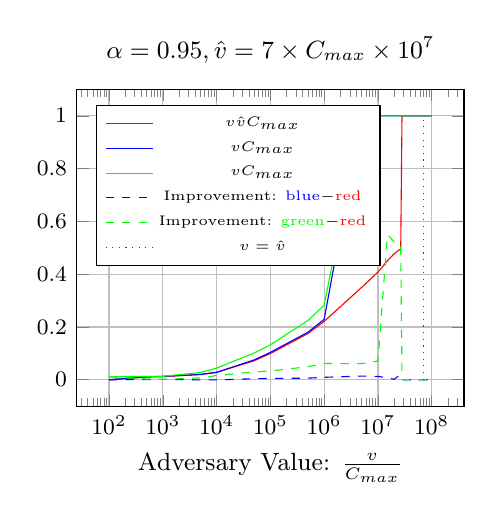
\begin{tikzpicture}[scale=1.0]  
   \begin{semilogxaxis}[
    title style={align=center},
    title={ {\small $\alpha=0.95, \hat{v} = 7\times C_{max} \times 10^7$ }},
       xlabel={Adversary Value: $\frac{v}{C_{max}}$},
ylabel shift = -3pt,
grid=major,
    small,
    cycle list = {{red, mark=none}, {blue, mark=none}, {green, mark=none},{blue, dashed, mark=none}, {green, dashed, mark=none},  {purple, dotted, mark=none}, {red, dashed, mark=none},{brown, dashed, mark=none} },
    legend style = {font=\tiny, at={(.05,.95)}, anchor=north west},
    legend entries = { $\PAdvCASH{v}{\hat{v}}{C_{max}}$, $\PAdvUnif{v}{C_{max}}$, $\PAdvDet{v}{C_{max}}$, Improvement: \textcolor{blue}{blue}$-$\textcolor{red}{red}, Improvement: \textcolor{green}{green}$-$\textcolor{red}{red}, $v = \hat{v}$  }
   ] 
   
    \addlegendimage{no markers, red, mark=square*}
    \addlegendimage{no markers, blue, mark=square*}
    \addlegendimage{no markers, green, mark=square*}
    \addlegendimage{no markers, dashed, blue}
    \addlegendimage{no markers, dashed, green}
    \addlegendimage{no markers, dotted, purple}
\addplot coordinates {  (100,0)  (500,0.0102822813124222)  (1000,0.0115631568630905)  (5000,0.0202897976021)  (10000,0.0283029983493156)  (50000,0.071791685890364)  (100000,0.0992383142594701)  (500000,0.175014737387696)  (1000000,0.221098434924485)  (5000000,0.35036457681152)  (10000000,0.407944399818817)  (15000000,0.450602587267483)  (20000000,0.477161630108202)  (25000000,0.492631378777674)  (26500000,0.492844202602487)  (28000000,0.999999999999971)  (30000000,0.999999999999971)  (70000000,0.999999999999971)  (100000000,0.999999999999971)  };


\addplot coordinates {  (100,0)  (500,0.0108687224894377)  (1000,0.0130192581998815)  (5000,0.0196877875530742)  (10000,0.0277625668318636)  (50000,0.0751253327190499)  (100000,0.103779181056781)  (500000,0.180114995472598)  (1000000,0.228825830589675)  (5000000,1)  (10000000,1)  (15000000,1)  (20000000,1)  (25000000,1)  (26500000,1)  (28000000,1)  (30000000,1)  (70000000,1)  (100000000,1)  };
\addplot coordinates {  (100,0.0108687224894377)  (500,0.0130192581998815)  (1000,0.0130192581998815)  (5000,0.0273838584095427)  (10000,0.0441510096695537)  (50000,0.101412040578669)  (100000,0.132372669808665)  (500000,0.224601121331902)  (1000000,0.282624504055384)  (5000000,1)  (10000000,1)  (15000000,1)  (20000000,1)  (25000000,1)  (26500000,1)  (28000000,1)  (30000000,1)  (70000000,1)  (100000000,1)  };
\addplot coordinates {  (100,0)  (500,0.000586441177015484)  (1000,0.001456101336791)  (5000,-0.000602010049025815)  (10000,-0.000540431517452054)  (50000,0.00382287259932285)  (100000,0.00504808644878749)  (500000,0.00604116345300501)  (1000000,0.00922406231680187)  (5000000,0.0138848603963081)  (10000000,0.0123729455738119)  (15000000,0.00774654963300692)  (20000000,0.00169175766987201)  (25000000,0.017118902086316)  (26500000,0.0169060782615023)  (28000000,2.89768209427166E-14)  (30000000,2.89768209427166E-14)  (70000000,2.89768209427166E-14)  (100000000,2.89768209427166E-14)  };
\addplot coordinates {  (100,0.0108687224894377)  (500,0.00273697688745928)  (1000,0.001456101336791)  (5000,0.00709406080744265)  (10000,0.0158480113202381)  (50000,0.0296203546883047)  (100000,0.0331343555491946)  (500000,0.0495863839442057)  (1000000,0.0615260691308984)  (5000000,0.0610035617281453)  (10000000,0.0709089879592568)  (15000000,0.549397412732517)  (20000000,0.522838369891798)  (25000000,0.507368621222326)  (26500000,0.507155797397513)  (28000000,2.89768209427166E-14)  (30000000,2.89768209427166E-14)  (70000000,2.89768209427166E-14)  (100000000,2.89768209427166E-14)  };

\addplot coordinates { (70000000, 0)  (70000000, 0.5)  (70000000, 1) };
   \end{semilogxaxis} 
  \end{tikzpicture}
  
\label{fig:YahooRobust1Results95}}


\subfloat[RockYou]{
    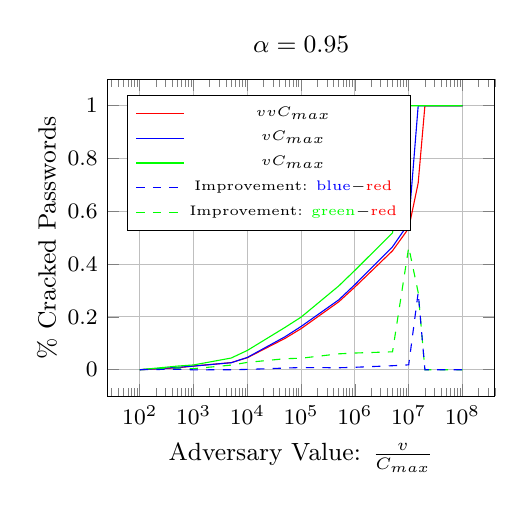
\begin{tikzpicture}[scale=1.0]  
   \begin{semilogxaxis}[
    title style={align=center},
    title={ {\small $\alpha=0.95$ }},
    xlabel={Adversary Value: $\frac{v}{C_{max}}$},
    ylabel={$\%$ Cracked Passwords},
    ylabel shift = -3pt,
grid=major,
    small,
    cycle list = {{red, mark=none}, {blue, mark=none}, {green, mark=none},{green, dashed, mark=none}, {blue, dashed, mark=none},  {blue, dashed, mark=none}, {red, dashed, mark=none},{brown, dashed, mark=none} },
    legend style = {font=\tiny, at={(.05,.95)}, anchor=north west},
    legend entries = { $\PAdvCASH{v}{v}{C_{max}}$, $\PAdvUnif{v}{C_{max}}$, $\PAdvDet{v}{C_{max}}$, Improvement: \textcolor{blue}{blue}$-$\textcolor{red}{red}, Improvement: \textcolor{green}{green}$-$\textcolor{red}{red}}
   ] 

    \addlegendimage{no markers, red, mark=square*}
    \addlegendimage{no markers, blue, mark=square*}
    \addlegendimage{no markers, green, mark=square*}
    \addlegendimage{no markers, dashed, blue}
    \addlegendimage{no markers, dashed, green}
\addplot coordinates {  (100,0)  (500,0.00703895183690825)  (1000,0.0141148535816532)  (5000,0.0267722121514504)  (10000,0.0454018848661649)  (50000,0.118439836836895)  (100000,0.155703757358036)  (500000,0.257165070416829)  (1000000,0.313403406714585)  (5000000,0.450583879056243)  (10000000,0.535863032524142)  (15000000,0.707445744531801)  (20000000,0.999999999999972)  (25000000,0.999999999999972)  (26500000,0.999999999999972)  (28000000,0.999999999999972)  (30000000,0.999999999999972)  (70000000,0.999999999999972)  (100000000,0.999999999999972)  };
\addplot coordinates {  (100,0)  (500,0.00891714075850031)  (1000,0.0136977788934083)  (5000,0.0265629142590948)  (10000,0.0465878576790853)  (50000,0.124664436714369)  (100000,0.164009427486493)  (500000,0.264563609156202)  (1000000,0.322603129466177)  (5000000,0.465731506185799)  (10000000,0.55428368364662)  (15000000,1)  (20000000,1)  (25000000,1)  (26500000,1)  (28000000,1)  (30000000,1)  (70000000,1)  (100000000,1)  };
\addplot coordinates {  (100,0)  (500,0.0136977788934083)  (1000,0.0180747779954648)  (5000,0.0441965417827129)  (10000,0.0730608733055595)  (50000,0.160089926850547)  (100000,0.199287847017616)  (500000,0.317302545367371)  (1000000,0.376634078642379)  (5000000,0.518411276766697)  (10000000,1)  (15000000,1)  (20000000,1)  (25000000,1)  (26500000,1)  (28000000,1)  (30000000,1)  (70000000,1)  (100000000,1)  };
\addplot coordinates {  (100,0)  (500,0.0066588270565)  (1000,0.0039599244138116)  (5000,0.0174243296312625)  (10000,0.0276589884393946)  (50000,0.0416500900136517)  (100000,0.0435840896595805)  (500000,0.0601374749505419)  (1000000,0.0632306719277944)  (5000000,0.0678273977104537)  (10000000,0.464136967475858)  (15000000,0.292554255468199)  (20000000,2.75335310107039E-14)  (25000000,2.75335310107039E-14)  (26500000,2.75335310107039E-14)  (28000000,2.75335310107039E-14)  (30000000,2.75335310107039E-14)  (70000000,2.75335310107039E-14)  (100000000,2.75335310107039E-14)  };
\addplot coordinates {  (100,0)  (500,0.00187818892159206)  (1000,-0.000417074688244912)  (5000,-0.000209297892355589)  (10000,0.00118597281292042)  (50000,0.00622459987747334)  (100000,0.00830567012845707)  (500000,0.00739853873937257)  (1000000,0.00919972275159225)  (5000000,0.0151476271295558)  (10000000,0.0184206511224776)  (15000000,0.292554255468199)  (20000000,2.75335310107039E-14)  (25000000,2.75335310107039E-14)  (26500000,2.75335310107039E-14)  (28000000,2.75335310107039E-14)  (30000000,2.75335310107039E-14)  (70000000,2.75335310107039E-14)  (100000000,2.75335310107039E-14)  };

   \end{semilogxaxis} 
  \end{tikzpicture}

\label{fig:RockYouResults95}}
\subfloat[RockYou: $\hat{v} \neq v$]{
    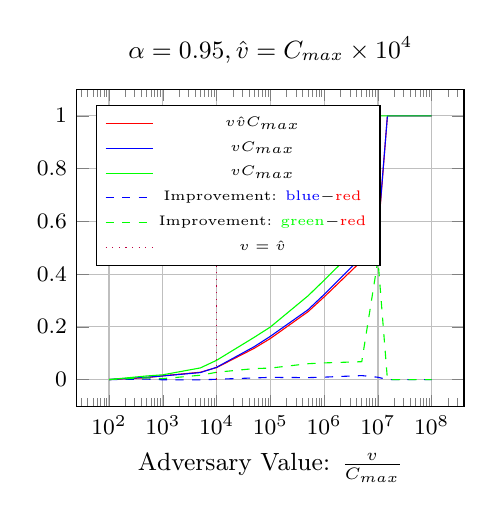
\begin{tikzpicture}[scale=1.0]  
   \begin{semilogxaxis}[
    title style={align=center},
    title={ {\small $\alpha=0.95, \hat{v} = C_{max}\times 10^4$ }},
       xlabel={Adversary Value: $\frac{v}{C_{max}}$},
ylabel shift = -3pt,
grid=major,
    small,
    cycle list = {{red, mark=none}, {blue, mark=none}, {green, mark=none},{blue, dashed, mark=none}, {green, dashed, mark=none},  {purple, dotted, mark=none}, {red, dashed, mark=none},{brown, dashed, mark=none} },
    legend style = {font=\tiny, at={(.05,.95)}, anchor=north west},
    legend entries = { $\PAdvCASH{v}{\hat{v}}{C_{max}}$, $\PAdvUnif{v}{C_{max}}$, $\PAdvDet{v}{C_{max}}$, Improvement: \textcolor{blue}{blue}$-$\textcolor{red}{red}, Improvement: \textcolor{green}{green}$-$\textcolor{red}{red}, $v = \hat{v}$  }
   ] 

    \addlegendimage{no markers, red, mark=square*}
    \addlegendimage{no markers, blue, mark=square*}
    \addlegendimage{no markers, green, mark=square*}
    \addlegendimage{no markers, dashed, blue}
    \addlegendimage{no markers, dashed, green}
    \addlegendimage{no markers, dotted, purple}
\addplot coordinates {  (100,0)  (500,0.00703895183690825)  (1000,0.0145237093081992)  (5000,0.0278110594326778)  (10000,0.0454018848661649)  (50000,0.118439836836895)  (100000,0.155703757358036)  (500000,0.257165070416829)  (1000000,0.313403406714585)  (5000000,0.450583879056243)  (10000000,0.545506415413783)  (15000000,0.999999999999972)  (20000000,0.999999999999972)  (25000000,0.999999999999972)  (26500000,0.999999999999972)  (27000000,0.999999999999972)  (27500000,0.999999999999972)  (28000000,0.999999999999972)  (29000000,0.999999999999972)  (30000000,0.999999999999972)  (70000000,0.999999999999972)  (100000000,0.999999999999972)  };
\addplot coordinates {  (100,0)  (500,0.00891714075850031)  (1000,0.0136977788934083)  (5000,0.0265629142590948)  (10000,0.0465878576790853)  (50000,0.124664436714369)  (100000,0.164009427486493)  (500000,0.264563609156202)  (1000000,0.322603129466177)  (5000000,0.465731506185799)  (10000000,0.55428368364662)  (15000000,1)  (20000000,1)  (25000000,1)  (26500000,1)  (27000000,1)  (27500000,1)  (28000000,1)  (29000000,1)  (30000000,1)  (70000000,1)  (100000000,1)  };
\addplot coordinates {  (100,0)  (500,0.0136977788934083)  (1000,0.0180747779954648)  (5000,0.0441965417827129)  (10000,0.0730608733055595)  (50000,0.160089926850547)  (100000,0.199287847017616)  (500000,0.317302545367371)  (1000000,0.376634078642379)  (5000000,0.518411276766697)  (10000000,1)  (15000000,1)  (20000000,1)  (25000000,1)  (26500000,1)  (27000000,1)  (27500000,1)  (28000000,1)  (29000000,1)  (30000000,1)  (70000000,1)  (100000000,1)  };

\addplot coordinates {  (100,0)  (500,0.00187818892159206)  (1000,-0.000825930414790916)  (5000,-0.00124814517358296)  (10000,0.00118597281292042)  (50000,0.00622459987747334)  (100000,0.00830567012845707)  (500000,0.00739853873937257)  (1000000,0.00919972275159225)  (5000000,0.0151476271295558)  (10000000,0.00877726823283698)  (15000000,2.75335310107039E-14)  (20000000,2.75335310107039E-14)  (25000000,2.75335310107039E-14)  (26500000,2.75335310107039E-14)  (27000000,2.75335310107039E-14)  (27500000,2.75335310107039E-14)  (28000000,2.75335310107039E-14)  (29000000,2.75335310107039E-14)  (30000000,2.75335310107039E-14)  (70000000,2.75335310107039E-14)  (100000000,2.75335310107039E-14)  };
\addplot coordinates {  (100,0)  (500,0.0066588270565)  (1000,0.00355106868726559)  (5000,0.0163854823500351)  (10000,0.0276589884393946)  (50000,0.0416500900136517)  (100000,0.0435840896595805)  (500000,0.0601374749505419)  (1000000,0.0632306719277944)  (5000000,0.0678273977104537)  (10000000,0.454493584586217)  (15000000,2.75335310107039E-14)  (20000000,2.75335310107039E-14)  (25000000,2.75335310107039E-14)  (26500000,2.75335310107039E-14)  (27000000,2.75335310107039E-14)  (27500000,2.75335310107039E-14)  (28000000,2.75335310107039E-14)  (29000000,2.75335310107039E-14)  (30000000,2.75335310107039E-14)  (70000000,2.75335310107039E-14)  (100000000,2.75335310107039E-14)  };


\addplot coordinates { (10000, 0)  (10000, 0.5)  (10000, 1) };


   \end{semilogxaxis} 
  \end{tikzpicture}
  
\label{fig:RockYouRobust2Results95}
}
\subfloat[RockYou: $\hat{v} \neq v$.]{
    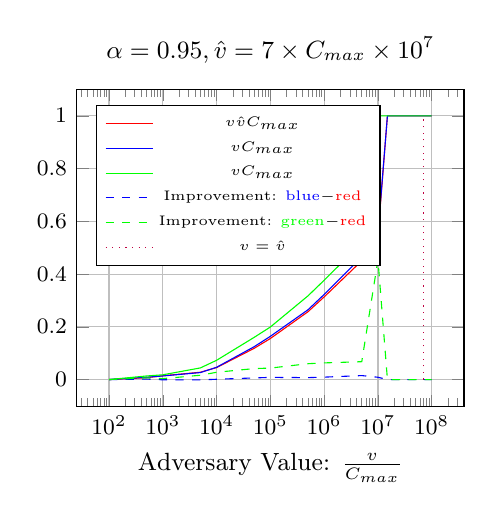
\begin{tikzpicture}[scale=1.0]  
   \begin{semilogxaxis}[
    title style={align=center},
    title={ {\small $\alpha=0.95, \hat{v} = 7\times C_{max} \times 10^7$ }},
       xlabel={Adversary Value: $\frac{v}{C_{max}}$},
ylabel shift = -3pt,
grid=major,
    small,
    cycle list = {{red, mark=none}, {blue, mark=none}, {green, mark=none},{blue, dashed, mark=none}, {green, dashed, mark=none},  {purple, dotted, mark=none}, {red, dashed, mark=none},{brown, dashed, mark=none} },
    legend style = {font=\tiny, at={(.05,.95)}, anchor=north west},
    legend entries = { $\PAdvCASH{v}{\hat{v}}{C_{max}}$, $\PAdvUnif{v}{C_{max}}$, $\PAdvDet{v}{C_{max}}$, Improvement: \textcolor{blue}{blue}$-$\textcolor{red}{red}, Improvement: \textcolor{green}{green}$-$\textcolor{red}{red}, $v = \hat{v}$  }
   ] 

    \addlegendimage{no markers, red, mark=square*}
    \addlegendimage{no markers, blue, mark=square*}
    \addlegendimage{no markers, green, mark=square*}
    \addlegendimage{no markers, dashed, blue}
    \addlegendimage{no markers, dashed, green}
    \addlegendimage{no markers, dotted, purple}
\addplot coordinates {  (100,0)  (500,0.00703895183690825)  (1000,0.0145237093081992)  (5000,0.0278110594326778)  (10000,0.0454018848661649)  (50000,0.118439836836895)  (100000,0.155703757358036)  (500000,0.257165070416829)  (1000000,0.313403406714585)  (5000000,0.450583879056243)  (10000000,0.545506415413783)  (15000000,0.999999999999972)  (20000000,0.999999999999972)  (25000000,0.999999999999972)  (26500000,0.999999999999972)  (27000000,0.999999999999972)  (27500000,0.999999999999972)  (28000000,0.999999999999972)  (29000000,0.999999999999972)  (30000000,0.999999999999972)  (70000000,0.999999999999972)  (100000000,0.999999999999972)  };

\addplot coordinates {  (100,0)  (500,0.00891714075850031)  (1000,0.0136977788934083)  (5000,0.0265629142590948)  (10000,0.0465878576790853)  (50000,0.124664436714369)  (100000,0.164009427486493)  (500000,0.264563609156202)  (1000000,0.322603129466177)  (5000000,0.465731506185799)  (10000000,0.55428368364662)  (15000000,1)  (20000000,1)  (25000000,1)  (26500000,1)  (27000000,1)  (27500000,1)  (28000000,1)  (29000000,1)  (30000000,1)  (70000000,1)  (100000000,1)  };
\addplot coordinates {  (100,0)  (500,0.0136977788934083)  (1000,0.0180747779954648)  (5000,0.0441965417827129)  (10000,0.0730608733055595)  (50000,0.160089926850547)  (100000,0.199287847017616)  (500000,0.317302545367371)  (1000000,0.376634078642379)  (5000000,0.518411276766697)  (10000000,1)  (15000000,1)  (20000000,1)  (25000000,1)  (26500000,1)  (27000000,1)  (27500000,1)  (28000000,1)  (29000000,1)  (30000000,1)  (70000000,1)  (100000000,1)  };


\addplot coordinates {  (100,0)  (500,0.00187818892159206)  (1000,-0.000825930414790916)  (5000,-0.00124814517358296)  (10000,0.00118597281292042)  (50000,0.00622459987747334)  (100000,0.00830567012845707)  (500000,0.00739853873937257)  (1000000,0.00919972275159225)  (5000000,0.0151476271295558)  (10000000,0.00877726823283698)  (15000000,2.75335310107039E-14)  (20000000,2.75335310107039E-14)  (25000000,2.75335310107039E-14)  (26500000,2.75335310107039E-14)  (27000000,2.75335310107039E-14)  (27500000,2.75335310107039E-14)  (28000000,2.75335310107039E-14)  (29000000,2.75335310107039E-14)  (30000000,2.75335310107039E-14)  (70000000,2.75335310107039E-14)  (100000000,2.75335310107039E-14)  };
\addplot coordinates {  (100,0)  (500,0.0066588270565)  (1000,0.00355106868726559)  (5000,0.0163854823500351)  (10000,0.0276589884393946)  (50000,0.0416500900136517)  (100000,0.0435840896595805)  (500000,0.0601374749505419)  (1000000,0.0632306719277944)  (5000000,0.0678273977104537)  (10000000,0.454493584586217)  (15000000,2.75335310107039E-14)  (20000000,2.75335310107039E-14)  (25000000,2.75335310107039E-14)  (26500000,2.75335310107039E-14)  (27000000,2.75335310107039E-14)  (27500000,2.75335310107039E-14)  (28000000,2.75335310107039E-14)  (29000000,2.75335310107039E-14)  (30000000,2.75335310107039E-14)  (70000000,2.75335310107039E-14)  (100000000,2.75335310107039E-14)  };

\addplot coordinates { (70000000, 0)  (70000000, 0.5)  (70000000, 1) };
   \end{semilogxaxis} 
  \end{tikzpicture}
  
\label{fig:RockYouRobust1Results95}
}
\caption{$\alpha=0.95$}

\end{figure}

\subsection{Discussion} 
In our experiments we varied the password correctness rate $\alpha \in \{0.9,0.95,1\}$. Intuitively, we expect for CASH to have a greater advantage over traditional key-stretching techniques when $\alpha$ is larger, but when $\alpha \rightarrow 0$ we should not expect for CASH or uniform-CASH to outperform deterministic key-stretching techniques because there is no advantage in making authentication costs asymmetric. It is easier for users to remember passwords that they use frequently\cite{Pimsleur1967,BS14,blockiSpacedRepetition} so we would expect for $\alpha$ to be larger for services that are used frequently (e.g., e-mail). This suggests that larger values of $\alpha$ (e.g., $\alpha = 0.9$ or $\alpha=0.95$) would be appropriate for many services because the users who authenticate most frequently would be the least likely to enter incorrect passwords. While different authentication servers might experience different failed login rates $1-\alpha$, we remark that it is reasonable to assume that the authentication server knows the value of $\alpha$ because it can monitor login attempts.


\paragraph{Estimating $v$} While our results suggest that CASH continues to perform well even if our estimate $\hat{v}$ of the adversary's value $v$ for cracked passwords is wrong, we would still recommend that an authentication server perform a careful economic analysis to obtain the estimate $\hat{v}$ before running Algorithm \ref{alg:HeuristicAlg2} to compute the CASH distribution $\tilde{p}$. The organization should take into account empirical data on the cost $\mathbf{Cost}\left(\mathbf{H}\right)$ of computing the underlying hash function as well as the market value of a cracked password. If possible, we recommend that the organization consider data from black market sales of passwords for similar types of  accounts (e.g., an adversary would likely value a cracked Bank of America password more than a cracked Twitter password). Symantec reports that cracked passwords are sold on the black market for $\$4$--$\$30$~\cite{passwordBlackMarket}. Thus, $\$30/\CostH$ might be a reasonable upper bound on the adversary's value for a cracked password (measured in \# of computations of $\Hash^k$). We would also strongly advocate for the use of memory hard functions instead of hash iteration to increase $\CostH$ effectively (see discussion in Section \ref{subsec:Traditional}). 


 \begin{figure}[!t]
\subfloat[Yahoo Dataset.]{
      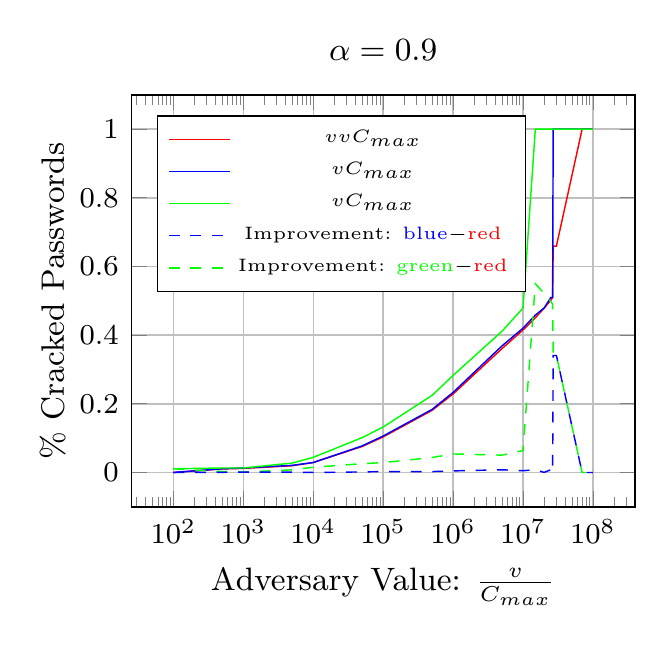
\begin{tikzpicture}[scale=1.3]  
   \begin{semilogxaxis}[
    title style={align=center},
    title={ {\small $\alpha=0.9$ }},
    xlabel={Adversary Value: $\frac{v}{C_{max}}$},
    ylabel={$\%$ Cracked Passwords},
    ylabel shift = -3pt,
grid=major,
    small,
    cycle list = {{red, mark=none}, {blue, mark=none}, {green, mark=none},{green, dashed, mark=none}, {blue, dashed, mark=none},  {blue, dashed, mark=none}, {red, dashed, mark=none},{brown, dashed, mark=none} },
    legend style = {font=\tiny, at={(.05,.95)}, anchor=north west},
    legend entries = { $\PAdvCASH{v}{v}{C_{max}}$, $\PAdvUnif{v}{C_{max}}$, $\PAdvDet{v}{C_{max}}$, Improvement: \textcolor{blue}{blue}$-$\textcolor{red}{red}, Improvement: \textcolor{green}{green}$-$\textcolor{red}{red}}
   ] 

    \addlegendimage{no markers, red, mark=square*}
    \addlegendimage{no markers, blue, mark=square*}
    \addlegendimage{no markers, green, mark=square*}
    \addlegendimage{no markers, dashed, blue}
    \addlegendimage{no markers, dashed, green}
\addplot coordinates {  (100,0)  (500,0.0103650003300184)  (1000,0.0118193070978086)  (5000,0.0196537617974582)  (10000,0.0289970884688705)  (50000,0.0757213976299667)  (100000,0.103595972530575)  (500000,0.181006843045768)  (1000000,0.228656981329561)  (5000000,0.360821094325625)  (10000000,0.415177925518485)  (15000000,0.450283451843314)  (20000000,0.47863343472216)  (25000000,0.501829516819531)  (26500000,0.509750280863969)  (27000000,0.659338193697864)  (27500000,0.659338193697864)  (28000000,0.659338193697864)  (29000000,0.659338193697864)  (30000000,0.659338193697864)  (70000000,0.999999999999979)  (100000000,0.999999999999979)  };
\addplot coordinates {  (100,0)  (500,0.0108687224894377)  (1000,0.0130192581998815)  (5000,0.0207614032035197)  (10000,0.0289970884688704)  (50000,0.0773727496772537)  (100000,0.106225338769438)  (500000,0.183571148129509)  (1000000,0.233240940214472)  (5000000,0.368658241037976)  (10000000,0.420317345392629)  (15000000,0.45834913690049)  (20000000,0.478853387778074)  (25000000,0.50975028086399)  (26500000,0.50975028086399)  (27000000,1)  (27500000,1)  (28000000,1)  (29000000,1)  (30000000,1)  (70000000,1)  (100000000,1)  };
\addplot coordinates {  (100,0.0108687224894377)  (500,0.0130192581998815)  (1000,0.0130192581998815)  (5000,0.0273838584095427)  (10000,0.0441510096695537)  (50000,0.101412040578669)  (100000,0.132372669808665)  (500000,0.224601121331902)  (1000000,0.282624504055384)  (5000000,0.411368138539665)  (10000000,0.478853387778074)  (15000000,1)  (20000000,1)  (25000000,1)  (26500000,1)  (27000000,1)  (27500000,1)  (28000000,1)  (29000000,1)  (30000000,1)  (70000000,1)  (100000000,1)  };
\addplot coordinates {  (100,0.0108687224894377)  (500,0.00265425786986305)  (1000,0.00119995110207291)  (5000,0.00773009661208442)  (10000,0.0151539212006832)  (50000,0.025690642948702)  (100000,0.0287766972780896)  (500000,0.0435942782861336)  (1000000,0.053967522725823)  (5000000,0.0505470442140399)  (10000000,0.0636754622595894)  (15000000,0.549716548156686)  (20000000,0.52136656527784)  (25000000,0.498170483180469)  (26500000,0.490249719136031)  (27000000,0.340661806302136)  (27500000,0.340661806302136)  (28000000,0.340661806302136)  (29000000,0.340661806302136)  (30000000,0.340661806302136)  (70000000,2.14273043752655E-14)  (100000000,2.14273043752655E-14)  };
\addplot coordinates {  (100,0)  (500,0.000503722159419252)  (1000,0.00119995110207291)  (5000,0.00110764140606149)  (10000,-1.49186218934005E-16)  (50000,0.00165135204728702)  (100000,0.00262936623886303)  (500000,0.00256430508374061)  (1000000,0.00458395888491178)  (5000000,0.00783714671235103)  (10000000,0.00513941987414457)  (15000000,0.0080656850571757)  (20000000,0.000219953055913658)  (25000000,0.00792076404445874)  (26500000,2.1094237467878E-14)  (27000000,0.340661806302136)  (27500000,0.340661806302136)  (28000000,0.340661806302136)  (29000000,0.340661806302136)  (30000000,0.340661806302136)  (70000000,2.14273043752655E-14)  (100000000,2.14273043752655E-14)  };


   \end{semilogxaxis} 
  \end{tikzpicture}
  
\label{fig:YahooResults90}}
\subfloat[RockYou Dataset.]{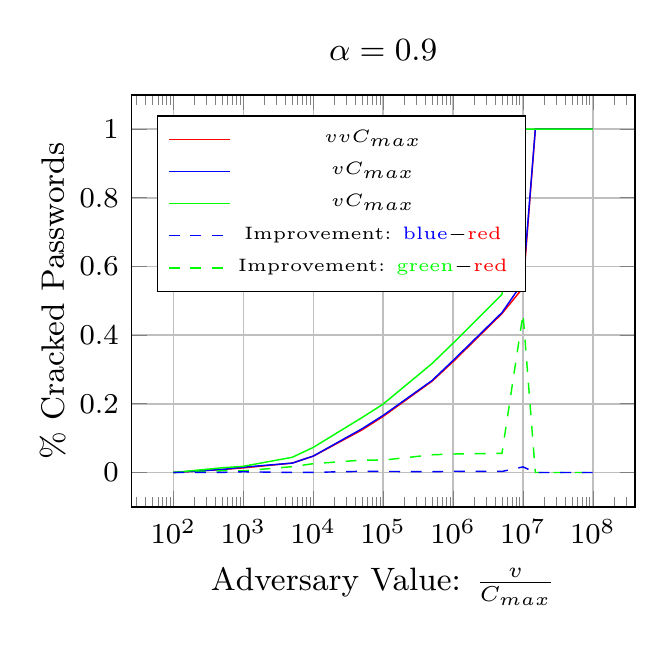
\begin{tikzpicture}[scale=1.3]  
   \begin{semilogxaxis}[
    title style={align=center},
    title={ {\small $\alpha=0.9$ }},
    xlabel={Adversary Value: $\frac{v}{C_{max}}$},
    ylabel={$\%$ Cracked Passwords},
    ylabel shift = -3pt,
grid=major,
    small,
    cycle list = {{red, mark=none}, {blue, mark=none}, {green, mark=none},{green, dashed, mark=none}, {blue, dashed, mark=none},  {blue, dashed, mark=none}, {red, dashed, mark=none},{brown, dashed, mark=none} },
    legend style = {font=\tiny, at={(.05,.95)}, anchor=north west},
    legend entries = { $\PAdvCASH{v}{v}{C_{max}}$, $\PAdvUnif{v}{C_{max}}$, $\PAdvDet{v}{C_{max}}$, Improvement: \textcolor{blue}{blue}$-$\textcolor{red}{red}, Improvement: \textcolor{green}{green}$-$\textcolor{red}{red}}
   ] 

    \addlegendimage{no markers, red, mark=square*}
    \addlegendimage{no markers, blue, mark=square*}
    \addlegendimage{no markers, green, mark=square*}
    \addlegendimage{no markers, dashed, blue}
    \addlegendimage{no markers, dashed, green}
\addplot coordinates {  (100,0)  (500,0.00859451942407725)  (1000,0.0133447400377569)  (5000,0.0272760303315716)  (10000,0.0474032707627518)  (50000,0.124170424428517)  (100000,0.163294928646465)  (500000,0.265801301128427)  (1000000,0.322799966527542)  (5000000,0.462803564928199)  (10000000,0.538000264865568)  (15000000,0.999999999999978)  (20000000,0.999999999999978)  (25000000,0.999999999999978)  (26500000,0.999999999999978)  (27000000,0.999999999999978)  (27500000,0.999999999999978)  (28000000,0.999999999999978)  (29000000,0.999999999999978)  (30000000,0.999999999999978)  (70000000,0.999999999999978)  (100000000,0.999999999999978)  };
\addplot coordinates {  (100,0)  (500,0.00891714075850031)  (1000,0.0155215770827253)  (5000,0.0272760303315717)  (10000,0.0478123623225905)  (50000,0.127514539286531)  (100000,0.166347957457673)  (500000,0.267932308139264)  (1000000,0.326354365380677)  (5000000,0.465731506185799)  (10000000,0.55428368364662)  (15000000,1)  (20000000,1)  (25000000,1)  (26500000,1)  (27000000,1)  (27500000,1)  (28000000,1)  (29000000,1)  (30000000,1)  (70000000,1)  (100000000,1)  };
\addplot coordinates {  (100,0)  (500,0.0136977788934083)  (1000,0.0180747779954648)  (5000,0.0441965417827129)  (10000,0.0730608733055595)  (50000,0.160089926850547)  (100000,0.199287847017616)  (500000,0.317302545367371)  (1000000,0.376634078642379)  (5000000,0.518411276766697)  (10000000,1)  (15000000,1)  (20000000,1)  (25000000,1)  (26500000,1)  (27000000,1)  (27500000,1)  (28000000,1)  (29000000,1)  (30000000,1)  (70000000,1)  (100000000,1)  };
\addplot coordinates {  (100,0)  (500,0.00510325946933101)  (1000,0.00473003795770787)  (5000,0.0169205114511413)  (10000,0.0256576025428077)  (50000,0.0359195024220297)  (100000,0.0359929183711517)  (500000,0.0515012442389441)  (1000000,0.0538341121148372)  (5000000,0.0556077118384979)  (10000000,0.461999735134432)  (15000000,2.22044604925031E-14)  (20000000,2.22044604925031E-14)  (25000000,2.22044604925031E-14)  (26500000,2.22044604925031E-14)  (27000000,2.22044604925031E-14)  (27500000,2.22044604925031E-14)  (28000000,2.22044604925031E-14)  (29000000,2.22044604925031E-14)  (30000000,2.22044604925031E-14)  (70000000,2.22044604925031E-14)  (100000000,2.22044604925031E-14)  };
\addplot coordinates {  (100,0)  (500,0.000322621334423063)  (1000,0.00217683704496837)  (5000,8.32667268468867E-17)  (10000,0.000409091559838717)  (50000,0.00334411485801335)  (100000,0.00305302881120795)  (500000,0.0021310070108374)  (1000000,0.00355439885313574)  (5000000,0.00292794125760004)  (10000000,0.0162834187810521)  (15000000,2.22044604925031E-14)  (20000000,2.22044604925031E-14)  (25000000,2.22044604925031E-14)  (26500000,2.22044604925031E-14)  (27000000,2.22044604925031E-14)  (27500000,2.22044604925031E-14)  (28000000,2.22044604925031E-14)  (29000000,2.22044604925031E-14)  (30000000,2.22044604925031E-14)  (70000000,2.22044604925031E-14)  (100000000,2.22044604925031E-14)  };


   \end{semilogxaxis} 
  \end{tikzpicture}
  
\label{fig:RockYouResults90}}
\centering
\caption{$\alpha = 0.9$.}
\end{figure}

\paragraph{Obtaining an Empirical Password Distribution} We remark that the specific CASH distributions we computed for the RockYou and Yahoo! datasets might not be optimal in other application settings because the underlying password distribution may vary across different contexts. For example, users might be more motivated to pick strong passwords for higher value accounts (e.g., bank accounts). Similarly, some organizations choose to restrict the passwords that a user may select (e.g., requiring upper and lower case letters). While these restrictions do not always result in stronger passwords~\cite{usability:compositionPolicies}, they can alter the underlying password distribution~\cite{blockiPasswordComposition}. While the underlying distribution may vary from context to context, we note that an authentication server could always follow the framework of Bonneau~\cite{bonneau2012science} and Blocki et al.~\cite{blocki2016differentially} to securely approximate the password distribution $p_1,\ldots,p_n$ of its own users. 

If an organization remains highly uncertain about value $v$ of a cracked password or about the empirical password distribution $p_1,\ldots, p_n$ then it may be prudent to adopt the uniform-CASH mechanism (e.g., \cite{manber1996simple}), which {\em always } performs at least as well as the traditional key-stretching approach.

\subsubsection{Experimental Limitations} \label{subsubsec:Limitations}
We remark that values of $\PAdvCASH{v}{\hat{v}}{C}$ that we compute in our experiments may be less realistic for larger values of $\frac{v}{\ServerCost{\alpha}}$ (e.g., $10^8$). The reason is that $p_i$, our empirical estimate of the probability of password $pwd_i$, will be too high for many of our unique passwords in the dataset. For example, consider a dedicated user who memorizes a truly random $20$ character string of upper and lower case letters. The true probability that any individual password guess matches the user's password would be at most $1/52^{20} \approx 1/\left(2.09 \times 10^{34} \right) $. However, if that password occurred in the RockYou dataset then our empirical estimate of this probability would be at least $1/\left(3.26\times 10^7\right)$. Developing improved techniques for estimating the true likelihood of unique password in a password frequency dataset is an important research direction.
